\documentclass[12pt,fleqn]{article}\usepackage[]{graphicx}\usepackage[]{color}
%% maxwidth is the original width if it is less than linewidth
%% otherwise use linewidth (to make sure the graphics do not exceed the margin)
\makeatletter
\def\maxwidth{ %
  \ifdim\Gin@nat@width>\linewidth
    \linewidth
  \else
    \Gin@nat@width
  \fi
}
\makeatother

\definecolor{fgcolor}{rgb}{0.345, 0.345, 0.345}
\newcommand{\hlnum}[1]{\textcolor[rgb]{0.686,0.059,0.569}{#1}}%
\newcommand{\hlstr}[1]{\textcolor[rgb]{0.192,0.494,0.8}{#1}}%
\newcommand{\hlcom}[1]{\textcolor[rgb]{0.678,0.584,0.686}{\textit{#1}}}%
\newcommand{\hlopt}[1]{\textcolor[rgb]{0,0,0}{#1}}%
\newcommand{\hlstd}[1]{\textcolor[rgb]{0.345,0.345,0.345}{#1}}%
\newcommand{\hlkwa}[1]{\textcolor[rgb]{0.161,0.373,0.58}{\textbf{#1}}}%
\newcommand{\hlkwb}[1]{\textcolor[rgb]{0.69,0.353,0.396}{#1}}%
\newcommand{\hlkwc}[1]{\textcolor[rgb]{0.333,0.667,0.333}{#1}}%
\newcommand{\hlkwd}[1]{\textcolor[rgb]{0.737,0.353,0.396}{\textbf{#1}}}%
\let\hlipl\hlkwb

\usepackage{framed}
\makeatletter
\newenvironment{kframe}{%
 \def\at@end@of@kframe{}%
 \ifinner\ifhmode%
  \def\at@end@of@kframe{\end{minipage}}%
  \begin{minipage}{\columnwidth}%
 \fi\fi%
 \def\FrameCommand##1{\hskip\@totalleftmargin \hskip-\fboxsep
 \colorbox{shadecolor}{##1}\hskip-\fboxsep
     % There is no \\@totalrightmargin, so:
     \hskip-\linewidth \hskip-\@totalleftmargin \hskip\columnwidth}%
 \MakeFramed {\advance\hsize-\width
   \@totalleftmargin\z@ \linewidth\hsize
   \@setminipage}}%
 {\par\unskip\endMakeFramed%
 \at@end@of@kframe}
\makeatother

\definecolor{shadecolor}{rgb}{.97, .97, .97}
\definecolor{messagecolor}{rgb}{0, 0, 0}
\definecolor{warningcolor}{rgb}{1, 0, 1}
\definecolor{errorcolor}{rgb}{1, 0, 0}
\newenvironment{knitrout}{}{} % an empty environment to be redefined in TeX

\usepackage{alltt}
\usepackage{pgfplots}
\pgfplotsset{compat=1.7}
\usepackage[margin=1in]{geometry}
\usepackage{amsmath,amsthm,amssymb,scrextend}
\usepackage{fancyhdr}
\pagestyle{fancy}
\DeclareMathOperator{\rng}{Rng}
\DeclareMathOperator{\dom}{Dom}
\newcommand{\R}{\mathbb R}
\newcommand{\cont}{\subseteq}
\newcommand{\N}{\mathbb N}
\newcommand{\Z}{\mathbb Z}
\usepackage{tikz}
\usepackage{pgfplots}
\usepackage{amsmath}
\usepackage[mathscr]{euscript}
\let\euscr\mathscr \let\mathscr\relax% just so we can load this and rsfs
\usepackage[scr]{rsfso}
\usepackage{amsthm}
\usepackage{amssymb}
\usepackage{multicol}
\usepackage[colorlinks=true, pdfstartview=FitV, linkcolor=blue,
citecolor=blue, urlcolor=blue]{hyperref}

\usepackage{enumerate} % enable \begin{enumerate}[1.]
\renewcommand{\labelenumi}{\alph{enumi}.} %first level: (a),(b)
\renewcommand{\labelenumii}{\roman{enumii}.} %second level: i,ii

\theoremstyle{definition}
\newtheorem*{sol}{Solution}
\newtheorem*{claim}{Claim}
\newtheorem{problem}{}
% ---------------------------------------------------------------------------------------------
\IfFileExists{upquote.sty}{\usepackage{upquote}}{}
\begin{document}
\lhead{GLM}
\chead{Zhijian Liu}
\rhead{\today}



% Just put your proofs in between the \begin{proof} and the \end{proof} statements!

\section*{Homework \#6}
\begin{enumerate}[1.]
  \setcounter{enumi}{1}
  % 2.
    \item Refer to the Pregnancy Duration Data (p. 609), repeat the analysis on p.613 (the response variable is treated as Nominal categorical) using R or other statistical software. Compare your results with the ones in the text (from Minitab). Are they the same? If not, what is the cause? Interpret the parameters in the context of the problem.
\begin{knitrout}
\definecolor{shadecolor}{rgb}{0.969, 0.969, 0.969}\color{fgcolor}\begin{kframe}
\begin{alltt}
\hlstd{reg2} \hlkwb{<-} \hlkwd{multinom}\hlstd{(}\hlkwd{cbind}\hlstd{(preg3,preg2,preg1)} \hlopt{~} \hlstd{.}\hlopt{-}\hlstd{preg,} \hlkwc{data} \hlstd{= df2)}
\end{alltt}
\begin{verbatim}
## # weights:  21 (12 variable)
## initial  value 112.058453 
## iter  10 value 84.619847
## final  value 84.337718 
## converged
\end{verbatim}
\begin{alltt}
\hlkwd{summary}\hlstd{(reg2)}
\end{alltt}
\begin{verbatim}
## Call:
## multinom(formula = cbind(preg3, preg2, preg1) ~ . - preg, data = df2)
## 
## Coefficients:
##       (Intercept)       nutri     age1     age3  alcohol  smoking
## preg2    3.958370 -0.04644903 2.913475 1.887550 1.067001 2.230492
## preg1    5.475147 -0.06541919 2.957028 2.059662 2.042900 2.452362
## 
## Std. Errors:
##       (Intercept)      nutri      age1      age3   alcohol   smoking
## preg2    1.941063 0.01488581 0.8575544 0.8088255 0.6495262 0.6681955
## preg1    2.271677 0.01823916 0.9644921 0.8947727 0.7097461 0.7315106
## 
## Residual Deviance: 168.6754 
## AIC: 192.6754
\end{verbatim}
\end{kframe}
\end{knitrout}
    The results are the same. Actually I set the $3^{rd}$ category of \texttt{preg} as the reference category to make them the same. After adjusting other factors, when nutrition status increases 1 unit, the odds of pregnancy duration in category 2 over category 3 will change by a factor of $e^{-0.046}$, and the odds of pregnancy duration in category 1 over category 3 will change by a factor of $e^{-0.065}$. Keeping other variables constant, when a mother's age change from age category 2 to age category 1, the odds of pregnancy duration in category 2 over category 3 will change by a factor of $e^{2.91}$. Similarly, interpretation for other parameters can be drawn according to the output.
  % 3.
    \item (8.2) The data in Table 8.5 are from an investigation into satisfaction with hous- ing conditions in Copenhagen (derived from Example W in Cox and Snell, 1981, from original data from Madsen, 1971). Residents in selected areas living in rented homes built between 1960 and 1968 were questioned about their satisfaction and the degree of contact with other residents. The data were tabulated by type of housing.\\
        In addition, test whether there is interaction effect between “type of housing” and “contact with other neighbors” on the response variable “satisfaction.”\\[-25pt]
    \begin{center}
      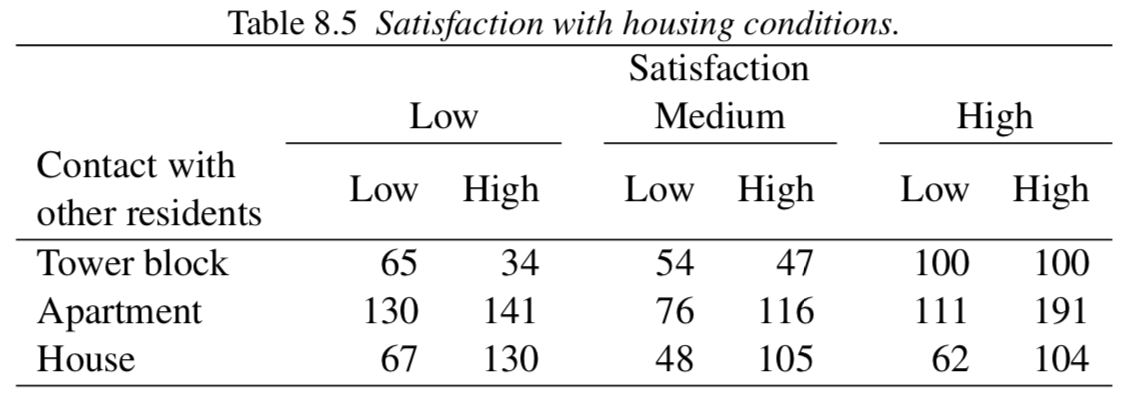
\includegraphics[width=0.7\linewidth]{table.png}
    \end{center}
      \begin{enumerate}[a.]
      % a.
        \item Summarize the data using appropriate tables of percentages to show the associations between levels of satisfaction and contact with other residents, levels of satisfaction and type of housing, and contact and type of housing.
\begin{knitrout}
\definecolor{shadecolor}{rgb}{0.969, 0.969, 0.969}\color{fgcolor}\begin{kframe}
\begin{verbatim}
##             contact
## satisfaction      high       low
##       high   0.2349792 0.1624033
##       low    0.1814396 0.1558596
##       medium 0.1594289 0.1058894
##             type
## satisfaction  Apartment      House TowerBlock
##       high   0.17965497 0.09875074 0.11897680
##       low    0.16121356 0.11719215 0.05889352
##       medium 0.11421773 0.09101725 0.06008328
##        type
## contact Apartment     House TowerBlock
##    high 0.2665080 0.2016657  0.1076740
##    low  0.1885782 0.1052945  0.1302796
\end{verbatim}
\end{kframe}
\end{knitrout}

      % b.
        \item Use nominal logistic regression to model associations between level of satisfaction and the other two variables. Obtain a parsimonious model that summarizes the patterns in the data.
\begin{knitrout}
\definecolor{shadecolor}{rgb}{0.969, 0.969, 0.969}\color{fgcolor}\begin{kframe}
\begin{alltt}
\hlstd{reg3} \hlkwb{<-} \hlkwd{multinom}\hlstd{(satisfaction} \hlopt{~} \hlstd{contact} \hlopt{+} \hlstd{type,} \hlkwc{weights} \hlstd{= frequency,} \hlkwc{data} \hlstd{= df3)}
\end{alltt}
\begin{verbatim}
## # weights:  15 (8 variable)
## initial  value 1846.767257 
## iter  10 value 1803.151908
## final  value 1802.740161 
## converged
\end{verbatim}
\begin{alltt}
\hlkwd{summary}\hlstd{(reg3)}
\end{alltt}
\begin{verbatim}
## Call:
## multinom(formula = satisfaction ~ contact + type, data = df3, 
##     weights = frequency)
## 
## Coefficients:
##        (Intercept) contactlow typeHouse typeTowerBlock
## low     -0.2474055  0.3282260 0.3040225     -0.6415725
## medium  -0.4654412  0.0322483 0.3736997     -0.2348298
## 
## Std. Errors:
##        (Intercept) contactlow typeHouse typeTowerBlock
## low     0.09783067  0.1181870 0.1351693       0.150077
## medium  0.10466300  0.1269192 0.1454812       0.154099
## 
## Residual Deviance: 3605.48 
## AIC: 3621.48
\end{verbatim}
\begin{alltt}
\hlstd{null} \hlkwb{<-} \hlkwd{multinom}\hlstd{(satisfaction} \hlopt{~} \hlnum{1}\hlstd{,} \hlkwc{weights} \hlstd{= frequency,} \hlkwc{data} \hlstd{= df3)}
\end{alltt}
\begin{verbatim}
## # weights:  6 (2 variable)
## initial  value 1846.767257 
## final  value 1824.438811 
## converged
\end{verbatim}
\begin{alltt}
\hlkwd{summary}\hlstd{(null)}
\end{alltt}
\begin{verbatim}
## Call:
## multinom(formula = satisfaction ~ 1, data = df3, weights = frequency)
## 
## Coefficients:
##        (Intercept)
## low     -0.1639289
## medium  -0.4039694
## 
## Std. Errors:
##        (Intercept)
## low     0.05710231
## medium  0.06114866
## 
## Residual Deviance: 3648.878 
## AIC: 3652.878
\end{verbatim}
\end{kframe}
\end{knitrout}
       \item[$\ast$] Test whether there is interaction effect between “type of housing” and “contact with other neighbors” on the response variable “satisfaction”.
\begin{knitrout}
\definecolor{shadecolor}{rgb}{0.969, 0.969, 0.969}\color{fgcolor}\begin{kframe}
\begin{alltt}
\hlstd{full} \hlkwb{<-}  \hlkwd{multinom}\hlstd{(satisfaction} \hlopt{~} \hlstd{contact}\hlopt{*}\hlstd{type,} \hlkwc{weights} \hlstd{= frequency,} \hlkwc{data} \hlstd{= df3)}
\end{alltt}
\begin{verbatim}
## # weights:  21 (12 variable)
## initial  value 1846.767257 
## iter  10 value 1800.889217
## final  value 1799.293647 
## converged
\end{verbatim}
\begin{alltt}
\hlkwd{c}\hlstd{(}\hlstr{'Chi^2'} \hlstd{= reg3}\hlopt{$}\hlstd{dev}\hlopt{-}\hlstd{full}\hlopt{$}\hlstd{dev,}\hlstr{'p-value'} \hlstd{=} \hlnum{1}\hlopt{-}\hlkwd{pchisq}\hlstd{(reg3}\hlopt{$}\hlstd{dev}\hlopt{-}\hlstd{full}\hlopt{$}\hlstd{dev,} \hlnum{10}\hlstd{))}
\end{alltt}
\begin{verbatim}
##     Chi^2   p-value 
## 6.8930278 0.7355037
\end{verbatim}
\begin{alltt}
\hlcom{# Df=12-2}
\end{alltt}
\end{kframe}
\end{knitrout}
        The likelihood ratio test indicates no interaction effect between “type of housing” and “contact with other neighbors” on the response variable “satisfaction”.
      \end{enumerate}
\end{enumerate}
\end{document}
